\section{Experiments}

In this section we discuss our experiments verifying the Linux-kernel 
Tree RCU implementation. We first describe several bug-injection
scenarios used in the experiments. Next, we report results of user-space runs
of the RCU model. Then we describe how verify our RCU model using CBMC. 
Finally, we discuss the experimental results.
%and then compare the results obtained with both approaches.
We performed our experiments on a 64-bit machine running Linux 3.19.8
with eight Intel Xeon 3.07\,GHz cores and 48\,GB of memory.

\subsection{Bug-Injection Scenarios} \label{sec:bug_cases}
Because we model non-preemptible Tree RCU, each CPU runs exactly one RCU task
as a separate thread.
Upon completion, each task increments a global counter \co{thread_cnt},
enabling the parent thread to verify the completion of all RCU tasks
using a statement \co{__CPROVER_assume(thread_cnt == 2)}.
The base case uses the example in Figure~\ref{fig:verify_rcu_gp}, including
its assertion \co{assert(r2 == 0 || r1 == 1)}.
This assertion does not hold when
RCU's fundamental safety guarantee is violated:
read-side critical sections cannot span grace
periods~\cite{DesnoyersTPDS12UserRCU}.
%
We also verify a \emph{weak form} of liveness by inserting an \co{assert(0)} 
after the \co{__CPROVER_assume(thread_cnt == 2)} statement.
This assertion cannot hold, and so it will be violated if at least one grace period completes.
Such a ``verification failure" is in fact the expected behavior for a correct RCU implementation. 
On the other hand, if the assertion is not violated, grace periods never complete, which indicates a liveness bug.

To validate our verification, we also run CBMC with the bug-injection scenarios 
described below,\footnote{Source code is available: \url{http://lxr.free-electrons.com/source/kernel/rcu/?v=4.3}}
which are simplified versions of bugs encountered in actual practice.
Bugs~2--6 are liveness checks and thus use the
aforementioned \co{assert(0)}, and the remaining scenarios are
safety checks which thus use the base-case assertion in
Figure~\ref{fig:verify_rcu_gp}.
% \comment{Lihao: we might explain each bug scenario in greater detail 
% assuming the readers aren't familiar with the code.}

\paragraph*{Bug 1}
This bug-injection scenario makes
the RCU update-side primitive \co{synchronize_rcu()} return immediately 
(line 523 in \co{tree_plugin.h}).
With this injected bug, updaters never wait for readers, which should
result in a safety violation, thus preventing
Figure~\ref{fig:verify_rcu_gp}'s assertion from holding.

\paragraph*{Bug 2}
The key idea behind this bug-injection scenario is to prevent individual
CPUs from realizing that quiescent states are needed, thus preventing
them from recording quiescent states. As a result, it prevents grace periods
from completing.
Specifically, in function \co{rcu_gp_init()}, for each \co{rcu_node}
structure in the combining tree,
we set the field \co{rnp->qsmask} to 0 instead of \co{rnp->qsmaskinit} (line 1889 in \co{tree.c}). 
Then when \co{rcu_process_callbacks()} is called, \co{rcu_check_quiescent_state()} will invoke
\co{__note_gp_changes()} that sets \co{rdp->qs_pending} to 0. Thus,  
\co{rcu_check_quiescent_state()} will return without calling \co{rcu_report_qs_rdp()},
preventing grace periods from completing.
This liveness violation should fail to trigger a violation of the end-of-execution
\co{assert(0)}.

\paragraph*{Bug 3}
This bug-injection scenario is a variation of Bug 2, in
which each CPU remains aware that quiescent states are required, but
incorrectly believes that it has already reported a quiescent state
for the current grace period.
To accomplish this,
in \co{__note_gp_changes()}, we clear \co{rnp->qsmask} by adding a statement
\co{rnp->qsmask &= ~rdp->grpmask;} in the last \co{if} code block (line 1739 in \co{tree.c}). 
Then function \co{rcu_report_qs_rnp()} never walks up the \co{rcu_node}
tree, resulting in a liveness violation as in Bug~2.

\paragraph*{Bug 4}
This bug-injection scenario is an alternative code change that gets the
same effect as does Bug~2.
For this alternative,
in \co{__note_gp_changes()}, we set the \co{rdp->qs_pending} field to 0 directly 
(line 1749 in \co{tree.c}). This is a variant of Bug 2 and thus also
a liveness violation.

\paragraph*{Bug 5}
In this bug-injection scenario, CPUs remain aware of the need for
quiescent states.
However, CPUs are prevented from recording their
quiescent states, thus preventing grace periods from ever completing.
To accomplish this, we modify
function \co{rcu_sched_qs()} to return immediately (line 246 in \co{tree.c}),
so that quiescent states are not recorded.
Grace periods therefore never complete, which constitutes a liveness
violation similar to Bug~2.

\paragraph*{Bug 6}
In this bug-injection scenario, CPUs are aware of the need for quiescent
states, and they also record them locally.
However, they are prevented from reporting them up the \co{rcu_node}
tree, which again prevents grace periods from ever completing.
This bug modifies
function \co{rcu_report_qs_rnp()} to return immediately (line 2227 in \co{tree.c}). 
This prevents RCU from walking up the \co{rcu_node} tree, thus preventing grace
periods from ending.
This is again a liveness violation similar to Bug~2.

\paragraph*{Bug 7}
Where Bug~6 prevents quiescent states from being reported up the
\co{rcu_node} tree, this bug-injection scenario causes quiescent
states to be reported up the tree prematurely, before all the
CPUs covered by a given subtree have all reported quiescent states.
To this end,
in \co{rcu_report_qs_rnp()}, we remove the \co{if}-block checking for
\co{rnp->qsmask != 0 || rcu_preempt_blocked_readers_cgp(rnp)} (line 2251 in \co{tree.c}). 
Then the tree-walking process will not stop until it reaches the root, resulting in 
too-short grace periods.
This is therefore a safety violation similar to Bug~1.

\noindent Bugs~2 and~3 would result in a too-short grace period given quiescent-state forcing, 
but such forcing falls outside the scope of this paper.


\subsection{Validating the RCU Model in User-Space}\label{sec:test_model}

\begin{table*}[tbh]
\centering
\scalebox{0.85}{%
\begin{tabular}{|l|r|r|r|c|r|c|} \hline
\multicolumn{1}{|c|}{\textbf{Scenario}} &
%\multicolumn{1}{c|}{\textbf{\#Total Runs}} &
\multicolumn{1}{c|}{\textbf{\#Successful Runs}} &
\multicolumn{1}{c|}{\textbf{\#Failing Runs}} &
\multicolumn{1}{c|}{\textbf{\#Timeouts}} &
\multicolumn{1}{c|}{\textbf{Max VM}} &
\multicolumn{1}{c|}{\textbf{Runtime}} &
\multicolumn{1}{c|}{\textbf{Result}} \\ \hline
Prove              & 1,000 (100.0\%) &     0 (0.0\%)   &     0 (0.0\%)   & 361.5\,MB & 3mins\,51s  & Safe                      \\ \hline 
Prove-GP           &     0 (0.0\%)   & 1,000 (100.0\%) &     0 (0.0\%)   & 361.5\,MB & 5mins\,9s   & End of GP Reachable       \\ \hline 
Bug 1              &   461 (46.1\%)  &   539 (53.9\%)  &     0 (0.0\%)   & 361.5\,MB & 5mins\,26s  & Assertion Violated        \\ \hline
Bug 2              &     0 (0.0\%)   &     0 (0.0\%)   & 1,000 (100.0\%) & 361.5\,MB & 16h\,40mins & End of GP Unreachable     \\ \hline
Bug 3              &     0 (0.0\%)   &     0 (0.0\%)   & 1,000 (100.0\%) & 361.5\,MB & 16h\,40mins & End of GP Unreachable     \\ \hline
Bug 4              &     0 (0.0\%)   &     0 (0.0\%)   & 1,000 (100.0\%) & 361.5\,MB & 16h\,40mins & End of GP Unreachable     \\ \hline
Bug 5              &     0 (0.0\%)   &     0 (0.0\%)   & 1,000 (100.0\%) & 361.5\,MB & 16h\,40mins & End of GP Unreachable     \\ \hline
Bug 6              &     0 (0.0\%)   &     0 (0.0\%)   & 1,000 (100.0\%) & 361.5\,MB & 16h\,40mins & End of GP Unreachable     \\ \hline
Bug 7              &     0 (0.0\%)   &     0 (0.0\%)   & 1,000 (100.0\%) & 361.5\,MB & 16h\,40mins & \mkcol{Safe (Bug Missed)} \\ \hline
Bug 7 (2 readers)  &   758 (75.8\%)  &   242 (24.2\%)  &     0 (0.0\%)   & 369.7\,MB & 4mins\,40s  & Assertion Violated        \\ \hline 
\end{tabular}
}
\caption{Experimental Results of Testing the RCU Model in User-Space}
\label{tab:results_run}
\end{table*}


%Lihao: as pointed out in Paul's recent emails, the bug-injection scenarios
%are probably a bit unfair to CBMC as they are fairly deterministic. So testing is 
%able to return the expected result for all of them. For future work, it might be 
%interesting to try more subtle ones such as removing fences, and compare CBMC 
%with RCU's regression test suite.
%To answer the question how difficult is it to detect the bugs we have
%injected using testing, we have executed our model in user space.  
To validate our RCU model before performing verification using CBMC, 
we executed it in user space. We performed 1000 runs for each scenario 
in Section~\ref{sec:bug_cases} using a 60\,s timeout to wait for the end of a 
grace period and a random delay between 0 to 1\,s in the RCU reader task.

The results are reported in Table~\ref{tab:results_run}.  Column 1 %and 2 
gives the verification scenarios. %and the total number of runs for each one of them, respectively.
Scenario Prove tests our RCU model without bug injection. Scenario Prove-GP 
tests a weak form of liveness by replacing Figure~\ref{fig:verify_rcu_gp}'s 
assertion with \co{assert(0)} as described in Section~\ref{sec:bug_cases}.
The next three columns present the number and the percentage of successful, 
failing, and timeout runs, respectively. The following two columns give the 
maximum memory consumption and the total runtime. The last column explains 
the results. 

As expected, for scenario Prove, the user program ran to completion
successfully in all runs.  For Prove-GP, it was able to detect the end of a
grace period by triggering an assertion violation in all the runs.  For
Bug~1, an assertion violation was triggered in 559 out of 1000 runs.  
%Thus, Bug~1 can be described as an ``easy'' bug.  By contrast, 
For Bugs 2--6, the user program timed out in all the runs, 
thus a grace period did not complete. %these bugs are difficult for testing.  
%\comment{Lihao: note that timeout is the expected behaviour for bugs 2--6. 
%See Section \ref{sec:bug_cases} for description of each bug-injection scenario.}
For Bug 7 with one reader thread, the testing harness failed to
trigger an assertion violation.  However, we were able to observe a failure in
242 out of 1000 runs with two reader threads.

% \comment{Lihao: shall we move the following paragraph to a more appropriate place, 
% e.g.~the end of either the CBMC or the Results and Discussion section.}
% I moved it to the end of the CBMC modeling section.  Might need to be
% summarized in results and discussion, definitely in conclusion.

%\comment{Lihao: item 9 in Paul's email}
%\comment{Lihao: there is a blog post \url{https://lkml.org/lkml/2009/9/1/229} 
%discussing to remove the timer interrupt and make the Linux kernel completely event-driven. 
%Paul, is this happening?}
%\\ \comment{Paul: Most of the motivation for that has been addressed
%by the \co{NO_HZ_FULL} work.  If it does happen, some of the work that
%RCU currently does from the scheduling-clock interrupt will need to be
%instead done by other means, for example, by hrtimer handlers.}

\subsection{Getting CBMC to work on Tree RCU} \label{sec:cbmc_on_rcu}

We have found that getting CBMC to work on our RCU model is non-trivial due
to Tree RCU's complexity combined with CBMC's bit-precise verification.  In
fact, early attempts resulted in SAT formulas that were so large that CBMC
ran out of memory.  After the optimizations described in the remainder of
this section, the largest formula contained around 90 million variables
and 450 million clauses, which enabled CBMC to run to completion.
%
% \comment{Paul: Do we have formula sizes from before this effort for
% purposes of comparison? Lihao: we do, but with different versions of the code. 
% For example, one version has 168 million variables and 738 million clauses. 
% Not sure which one to use, similar to the situation in the next comment.}

First, instead of placing the scheduling-clock interrupt in its own thread,
we invoke functions \co{rcu_note_context_switch()} and
\co{rcu_process_callbacks()} directly, as described in
Section~\ref{sec:model_irq}.  Also, we invoke
\co{__note_gp_changes()} from \co{rcu_gp_init()} to notify each CPU of a new
grace period, instead of invoking \co{rcu_process_callbacks()}.
%
%These changes reduced CBMC's common-case runtime from more than 24 hours to less than 10 hours.
% \comment{Paul: Can we provide this sort of blow-by-blow result for all steps?
% If not, should we should remove this one?
% Or give a qualitative comparision: ``Before applying this optimization,
% CBMC ran out of memory before completing the formula.'' Lihao: let's do the latter.}

Second, the support for linked lists in CBMC version 5.4 is limited,
resulting in unreachable code in CBMC's symbolic execution. Thus, we
stubbed all the list-related code in our RCU model, including those for
callback handling.

Third, CBMC's structure-pointer and array encodings result in large formulas
and long formula-generation times.  Our focus on the RCU-sched flavor
allowed us to eliminate RCU-BH's data structures and trivialize the
\co{for_each_rcu_flavor()} flavor-traversal loops.  Our focus on small
numbers of CPUs meant that RCU-sched's \co{rcu_node} tree contained only a
root node, so we also trivialized the \co{rcu_for_each_node_breadth_first()}
loops traversing this tree.

Fourth, CBMC unwinds each loop to the depth specified in its command line
option \co{--unwind}, even when the actual loop depth is smaller.  This
unnecessarily increases formula size, especially for loops containing
intricate RCU code. Since loops in our model can be decided at compile time, 
we therefore used the command line option \co{--unwindset} to specify 
unwinding depths for each individual loop.

Finally, since our test harness only requires one \co{rcu_node} structure
and two \co{rcu_data} structures, we can use 32-bit encodings for \co{int},
\co{long}, and pointers by using the command line option \co{--ILP32}.  This
reduces CBMC's formula size by half compared to the 64-bit default.


\subsection{Results and Discussion}

Table~\ref{tab:results_cbmc} presents the results of our experiments
applying CBMC version~5.4 to verify our RCU model.
Scenario Prove verifies our RCU model without
bug injection over Sequential Consistency (SC).  We also exercise the model
over the weak memory models TSO and PSO in scenarios Prove-TSO and Prove-PSO, 
respectively.  Scenario Prove-GP performs the same reachability check as in 
Section~\ref{sec:test_model} over SC.
%by replacing Figure~\ref{fig:verify_rcu_gp}'s assertion with \co{assert(0)} 
%as described in Section~\ref{sec:bug_cases}, which serves as a reachability check. 
We perform the same reachability verification over TSO
and PSO in scenarios Prove-GP-TSO and Prove-GP-PSO, respectively.  Scenarios
Bug~1--7 are the bug-injection scenarios discussed in
Section~\ref{sec:bug_cases}, and are verified over SC, TSO and PSO.  Columns
2--4 give the number of constraints (symbolic program expressions and
partial orders), variables, and clauses of the generated
formula.  The next three columns give the maximum (virtual) memory
consumption, solver runtime, and total runtime of our experiments.  The
final column gives the verification result.

% \comment{Lihao: the footnote in results.tex for bug 7 with 2 reader threads doesn't display?}
% I changed the footnote to text following the table.
% \comment{Lihao: we only use this more powerful machine to run bug 7 with 2 readers, 
% hence footnote seems more appropriate.}
% OK, I created a special within-table footnote.  ;-)

\begin{table*}[tbh]
\centering
\scalebox{0.85}{%
\begin{tabular}{|l|c|c|r|r|r|r|c|} \hline
\multicolumn{1}{|c|}{\textbf{Scenario}} &
\multicolumn{1}{c|}{\textbf{\#Constraints}} &
\multicolumn{1}{c|}{\textbf{\#Variables}} &
\multicolumn{1}{c|}{\textbf{\#Clauses}} &
\multicolumn{1}{c|}{\textbf{Max VM}} &
\multicolumn{1}{c|}{\textbf{Solver Time}} &
\multicolumn{1}{c|}{\textbf{Total Time}} &
\multicolumn{1}{c|}{\textbf{Result}} \\ \hline
Prove             &  5,279,600 & 30,085,337 & 149,758,548 & 23.27\,GB &  9h\,24mins &  9h\,36mins & Safe \\ \hline
Prove-TSO         &  5,646,959 & 42,042,386 & 210,708,442 & 34.00\,GB & 10h\,51mins & 11h\,4mins  & Safe \\ \hline
Prove-PSO         &  5,617,154 & 41,327,066 & 207,042,629 & 33.76\,GB & 11h\,23mins & 11h\,36mins & Safe \\ \hline
Prove-GP          &  5,476,540 & 30,655,428 & 152,743,545 & 23.90\,GB &  3h\,52mins &  4h\,5mins  & End of GP Reachable \\ \hline
Prove-GP-TSO      &  5,646,940 & 42,041,740 & 210,705,615 & 34.00\,GB & 13h\,1mins  & 13h\,14mins & End of GP Reachable \\ \hline
Prove-GP-PSO      &  5,617,135 & 41,326,420 & 207,039,802 & 33.76\,GB &  8h\,24mins &  8h\,37mins & End of GP Reachable \\ \hline
Bug 1             &  1,343,449 & 11,719,966 &  56,027,980 &  8.24\,GB &      31mins &      33mins & Assertion Violated \\ \hline
Bug 1-TSO         &  1,540,645 & 17,120,555 &  83,392,397 & 12.60\,GB &      53mins &      56mins & Assertion Violated \\ \hline
Bug 1-PSO         &  1,514,657 & 16,548,819 &  80,481,851 & 12.42\,GB &      46mins &      48mins & Assertion Violated \\ \hline
Bug 2             &  5,279,584 & 30,056,615 & 149,643,492 & 23.26\,GB &  4h\,25mins &  4h\,37mins & End of GP Unreachable \\ \hline
Bug 2-TSO         &  5,646,940 & 42,013,372 & 210,592,015 & 34.01\,GB &  9h\,57mins & 10h\,10mins & End of GP Unreachable \\ \hline
Bug 2-PSO         &  5,617,135 & 41,298,052 & 206,926,202 & 33.75\,GB &  8h\,51mins &  9h\,4mins & End of GP Unreachable \\ \hline
Bug 3             &  6,374,373 & 34,856,577 & 174,131,331 & 28.04\,GB &  7h\,11mins &  7h\,25mins & End of GP Unreachable \\ \hline
Bug 3-TSO         &  6,805,631 & 48,788,433 & 245,157,184 & 41.18\,GB & 19h\,40mins & 19h\,55mins & End of GP Unreachable \\ \hline
Bug 3-PSO         &  6,773,763 & 48,023,601 & 241,237,629 & 40.95\,GB & 19h\,19mins & 19h\,35mins & End of GP Unreachable \\ \hline
Bug 4             &  4,847,980 & 27,804,363 & 138,197,043 & 22.18\,GB &  4h\,3mins  &  4h\,14mins & End of GP Unreachable \\ \hline
Bug 4-TSO         &  5,170,928 & 38,480,891 & 192,605,939 & 31.49\,GB &  8h\,18mins &  8h\,30mins & End of GP Unreachable \\ \hline
Bug 4-PSO         &  5,141,123 & 37,765,571 & 188,940,126 & 31.27\,GB &  8h\,14mins &  8h\,26mins & End of GP Unreachable \\ \hline
Bug 5             &  5,161,874 & 29,510,828 & 146,787,005 & 23.02\,GB &  4h\,6mins  &  4h\,18mins & End of GP Unreachable \\ \hline
Bug 5-TSO         &  5,522,168 & 41,239,083 & 206,569,643 & 33.65\,GB &  5h\,46mins &  5h\,59mins & End of GP Unreachable \\ \hline
Bug 5-PSO         &  5,492,607 & 40,529,619 & 202,933,839 & 33.04\,GB &  5h\,42mins &  5h\,55mins & End of GP Unreachable \\ \hline
Bug 6             &  1,410,495 & 13,165,176 &  63,302,559 &  9.03\,GB &      19mins &      21mins & End of GP Unreachable \\ \hline
Bug 6-TSO         &  1,541,937 & 17,286,058 &  84,131,818 & 12.59\,GB &  1h\,32mins &  1h\,33mins & End of GP Unreachable \\ \hline
Bug 6-PSO         &  1,518,307 & 16,766,198 &  81,485,361 & 12.44\,GB &  1h\,22mins &  1h\,24mins & End of GP Unreachable \\ \hline
Bug 7             &  5,022,249 & 29,242,760 & 145,389,516 & 22.87\,GB &  8h\,48mins &  9h         & \mkcol{Safe (Bug Missed)} \\ \hline
Bug 7-TSO         &  5,201,744 & 40,139,251 & 200,857,404 & 31.93\,GB & 11h\,6mins  & 11h\,18mins & Assertion Violated \\ \hline
Bug 7-PSO         &  5,172,720 & 39,442,675 & 197,287,644 & 31.71\,GB & 11h\,32mins & 11h\,44mins & Assertion Violated \\ \hline
Bug 7 (2 readers) $^*$
                  & 15,165,557 & 71,205,400 & 359,021,922 & 59.07\,GB & 19h\,2mins  & 19h\,40mins & Assertion Violated \\ \hline
Bug 7-TSO (2 readers) $^*$
                  & 15,691,102 & 90,444,903 & 456,973,933 & 74.80\,GB & 78h\,12mins & 78h\,53mins & Assertion Violated \\ \hline
Bug 7-PSO (2 readers) $^*$
                  & 15,647,504 & 89,398,551 & 451,611,664 & 74.51\,GB & 84h\,21mins & 85h\,2mins  & \mkcol{Solver Out of Memory} \\ \hline
\end{tabular}
}
\vspace*{0.03cm} \\
\raggedright
\centering\footnotesize * This experiment was performed on a 64-bit machine running Linux 3.19.8 with twelve Intel Xeon 2.40\,GHz cores and 96\,GB of main memory
\vspace*{0.05cm}
\caption{Experimental Results of CBMC}
\label{tab:results_cbmc}
\end{table*}


Since Tree RCU's implementation in the Linux kernel is sophisticated, its test suite
is non-trivial~\cite{PaulMcKenney2005rcutorture}, comprising several thousand
lines of code.
% \comment{Paul, any reference I can cite for Tree RCU testing?} 
Therefore, it comes as little surprise that its verification is 
challenging.

In our experiments, CBMC returned all the expected results except
for Bug~7, for which it failed to report a violation of the
assertion \co{assert(r2 == 0 || r1 == 1)} with one RCU reader thread running
over SC.  This failure was due to the approximation of the
scheduling-clock interrupt by a direct function call,
as described in Section~\ref{sec:model_rcu}. 
% \comment{Lihao: should it be 'under-approximation'?  It can happen more
% frequently than the number of calls in our model.  I suggest we just use the
% word 'approximation'.}
However, CBMC did report a violation of the assertion
either when two RCU reader threads were present or when run over
TSO or PSO.
All of these cases decrease determinism,
which in turn more faithfully model non-deterministic
scheduling-clock interrupts, allowing the assertion to be violated.
% \comment{Lihao: shall we briefly explain why it's
% possible for TSO and PSO to detect bug 7 with one reader thread?}
%\comment{Lihao: briefly compare CBMC's results with the user-space program.}

CBMC took more than 9 hours to verify our model over SC (scenario Prove). 
The resulting SAT formulas have more than 5m
constraints, 30m variables and 149m clauses, and occupy
23\,GB of memory.  The formulas for scenarios Prove-TSO and
Prove-PSO are about
40\% larger than the scenario Prove.  They have more than 40m
variables and 200m clauses, and took more than 11 hours and 33\,GB
memory to solve.
Although this verification consumed considerable memory
and CPU, it verified all possible executions and
reorderings permitted by TSO and PSO,
a tiny subset of which are reached by
the \co{rcutorture} test suite.

CBMC proved that grace periods can end (i.e., \co{assert(0)} is
violated), over SC (Prove-GP), TSO (Prove-GP-TSO), and PSO
(Prove-GP-PSO).  The sizes of resulting formulas and memory consumption
are similar to those of the three Prove scenarios.
However, it took CBMC only about 4, 13, and 8.5 hours to find an
violation of \co{assert(0)} in Prove-GP, Prove-GP-TSO, and Prove-GP-PSO, respectively.

For the bug-injection scenarios described in Section~\ref{sec:bug_cases}, CBMC
was able to return the expected results in all scenarios over SC except for Bug~7,
as noted earlier.
The formula size varies from scenarios to
scenarios, with 27m--35m variables and 138m--174m
clauses.  The runtime was 4--9 hours and memory consumption exceeded
22\,GB.  The exceptions are Bugs~1 and 6, which have fewer than
14m variables and 64m clauses, and took less than 35 mins and
about 9\,GB of memory to solve.  This reduction was due to the large amount
of code removed by the bug injections in these scenarios.

% Lihao: include this in PhD thesis
\begin{figure}[tbp]
\centering
\captionsetup{justification=centering}
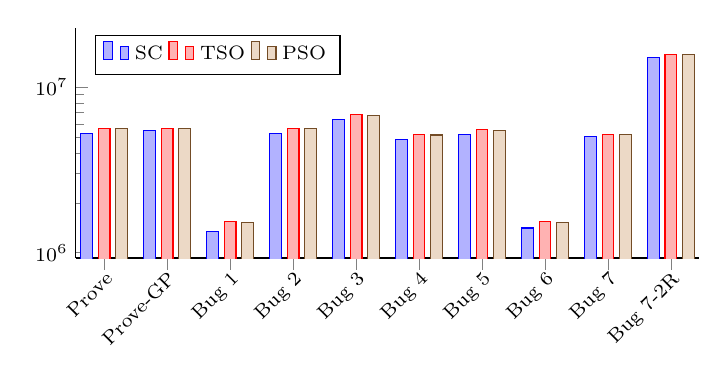
\begin{tikzpicture}
\scriptsize
\begin{axis}[
  ybar,
  bar width=0.15cm,
  height=4.5cm,
  width=9.5cm,
  axis lines*=left, % remove lines in the background
  ymode=log,
  %ylabel=Number of constraints,
  symbolic x coords={Prove, Prove-GP, Bug 1, Bug 2, Bug 3, 
                     Bug 4, Bug 5, Bug 6, Bug 7, Bug 7-2R,
                    },
  xtick=data,
  %nodes near coords, % numbers displayed above the bars
  %every node near coord/.append style={font=\small, rotate=90, anchor=west},
  xticklabel style={
    inner sep=0pt,
    anchor=north east,
    rotate=45
  },
  %enlargelimits=0.15,
  enlarge y limits=0.15, % space relative to the height of the plot
  enlarge x limits=0.05, % space relative to the width of the plot
  legend style={
    %anchor=north, at={(0.5, -0.9)}, % legend location
    legend pos=north west,
    legend columns=-1,
    font=\scriptsize},
]

\addplot % SC
  coordinates {(Prove, 5279600) (Prove-GP, 5476540)
               (Bug 1, 1343449) (Bug 2, 5279584) (Bug 3, 6374373)
               (Bug 4, 4847980) (Bug 5, 5161874) (Bug 6, 1410495)
               (Bug 7, 5022249) (Bug 7-2R, 15165557)
              };

\addplot % TSO 
  coordinates {(Prove, 5646959) (Prove-GP, 5646940)
               (Bug 1, 1540645) (Bug 2, 5646940) (Bug 3, 6805631)
               (Bug 4, 5170928) (Bug 5, 5522168) (Bug 6, 1541937)
               (Bug 7, 5201744) (Bug 7-2R, 15691102)
              };


\addplot % PSO
  coordinates {(Prove, 5617154) (Prove-GP, 5617135)
               (Bug 1, 1514657) (Bug 2, 5617135) (Bug 3, 6773763)
               (Bug 4, 5141123) (Bug 5, 5492607) (Bug 6, 1518307)
               (Bug 7, 5172720) (Bug 7-2R, 15647504)
              };

\legend{SC, TSO, PSO}
\end{axis}
\end{tikzpicture}

\caption{Number of Constraints in the SAT Formulas}
\label{fig:barchart_sat_constr}
\end{figure}

\begin{figure}[tbp]
\centering
\captionsetup{justification=centering}
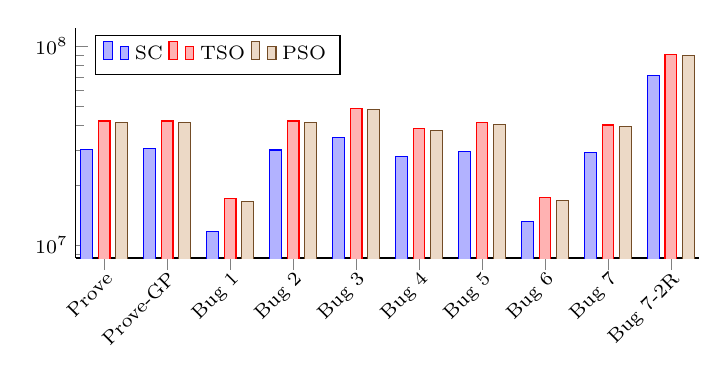
\begin{tikzpicture}
\scriptsize
\begin{axis}[
  ybar,
  bar width=0.15cm,
  height=4.5cm,
  width=9.5cm,
  axis lines*=left, % remove lines in the background
  ymode=log,
  %ylabel=Number of variables,
  symbolic x coords={Prove, Prove-GP, Bug 1, Bug 2, Bug 3, 
                     Bug 4, Bug 5, Bug 6, Bug 7, Bug 7-2R,
                    },
  xtick=data,
  %nodes near coords, % numbers displayed above the bars
  %every node near coord/.append style={font=\small, rotate=90, anchor=west},
  xticklabel style={
    inner sep=0pt,
    anchor=north east,
    rotate=45
  },
  %enlargelimits=0.15,
  enlarge y limits=0.15, % space relative to the height of the plot
  enlarge x limits=0.05, % space relative to the width of the plot
  legend style={
    %anchor=north, at={(0.5, -0.9)}, % legend location
    legend pos=north west,
    legend columns=-1,
    font=\scriptsize},
]

\addplot % SC
  coordinates {(Prove, 30085337) (Prove-GP, 30655428)
               (Bug 1, 11719966) (Bug 2, 30056615) (Bug 3, 34856577)
               (Bug 4, 27804363) (Bug 5, 29510828) (Bug 6, 13165176)
               (Bug 7, 29242760) (Bug 7-2R, 71205400)
              };

\addplot % TSO 
  coordinates {(Prove, 42042386) (Prove-GP, 42041740)
               (Bug 1, 17120555) (Bug 2, 42013372) (Bug 3, 48788433)
               (Bug 4, 38480891) (Bug 5, 41239083) (Bug 6, 17286058)
               (Bug 7, 40139251) (Bug 7-2R, 90444903)
              };


\addplot % PSO
  coordinates {(Prove, 41327066) (Prove-GP, 41326420)
               (Bug 1, 16548819) (Bug 2, 41298052) (Bug 3, 48023601)
               (Bug 4, 37765571) (Bug 5, 40529619) (Bug 6, 16766198)
               (Bug 7, 39442675) (Bug 7-2R, 89398551)
              };

\legend{SC, TSO, PSO}
\end{axis}
\end{tikzpicture}

\caption{Number of Variables in the SAT Formulas}
\label{fig:barchart_sat_var}
\end{figure}

\begin{figure}[tbp]
\centering
\captionsetup{justification=centering}
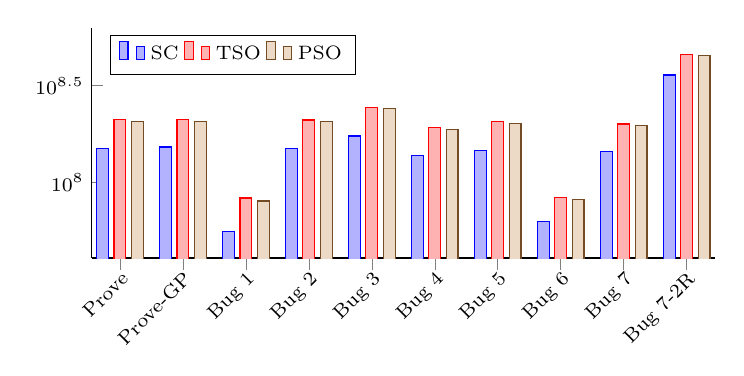
\begin{tikzpicture}
\scriptsize
\begin{axis}[
  ybar,
  bar width=0.15cm,
  height=4.5cm,
  width=9.5cm,
  axis lines*=left, % remove lines in the background
  ymode=log,
  %ylabel=Number of clauses,
  symbolic x coords={Prove, Prove-GP, Bug 1, Bug 2, Bug 3, 
                     Bug 4, Bug 5, Bug 6, Bug 7, Bug 7-2R,
                    },
  xtick=data,
  %nodes near coords, % numbers displayed above the bars
  %every node near coord/.append style={font=\small, rotate=90, anchor=west},
  xticklabel style={
    inner sep=0pt,
    anchor=north east,
    rotate=45
  },
  %enlargelimits=0.15,
  enlarge y limits=0.15, % space relative to the height of the plot
  enlarge x limits=0.05, % space relative to the width of the plot
  legend style={
    %anchor=north, at={(0.5, -0.9)}, % legend location
    legend pos=north west,
    legend columns=-1,
    font=\scriptsize},
]

\addplot % SC
  coordinates {(Prove, 149758548) (Prove-GP, 152743545)
               (Bug 1, 56027980) (Bug 2, 149643492) (Bug 3, 174131331)
               (Bug 4, 138197043) (Bug 5, 146787005) (Bug 6, 63302559)
               (Bug 7, 145389516) (Bug 7-2R, 359021922)
              };

\addplot % TSO 
  coordinates {(Prove, 210708442) (Prove-GP, 210705615)
               (Bug 1, 83392397) (Bug 2, 210592015) (Bug 3, 245157184)
               (Bug 4, 192605939) (Bug 5, 206569643) (Bug 6, 84131818)
               (Bug 7, 200857404) (Bug 7-2R, 456973933)
              };

\addplot % PSO
  coordinates {(Prove, 207042629) (Prove-GP, 207039802)
               (Bug 1, 80481851) (Bug 2, 206926202) (Bug 3, 241237629)
               (Bug 4, 188940126) (Bug 5, 202933839) (Bug 6, 81485361)
               (Bug 7, 197287644) (Bug 7-2R, 451611664)
              };

\legend{SC, TSO, PSO}
\end{axis}
\end{tikzpicture}

\caption{Number of Clauses in the SAT Formulas}
\label{fig:barchart_sat_clause}
\end{figure}

\begin{figure}[tbp]
\centering
\captionsetup{justification=centering}
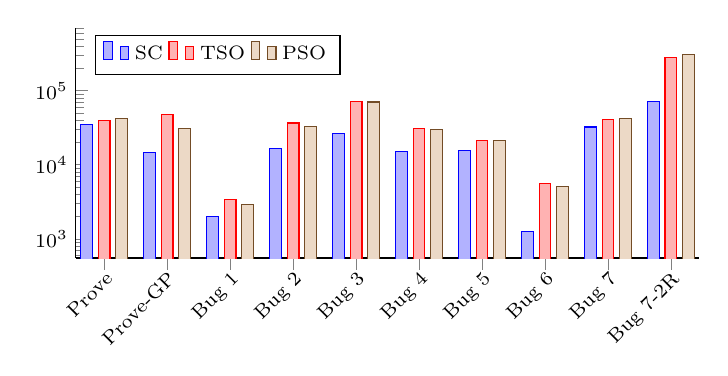
\begin{tikzpicture}
\scriptsize
\begin{axis}[
  ybar,
  bar width=0.15cm,
  height=4.5cm,
  width=9.5cm,
  axis lines*=left, % remove lines in the background
  ymode=log,
  %ylabel=Total runtime (seconds),
  symbolic x coords={Prove, Prove-GP, Bug 1, Bug 2, Bug 3, 
                     Bug 4, Bug 5, Bug 6, Bug 7, Bug 7-2R,
                    },
  xtick=data,
  %nodes near coords, % numbers displayed above the bars
  %every node near coord/.append style={font=\small, rotate=90, anchor=west},
  xticklabel style={
    inner sep=0pt,
    anchor=north east,
    rotate=45
  },
  %enlargelimits=0.15,
  enlarge y limits=0.15, % space relative to the height of the plot
  enlarge x limits=0.05, % space relative to the width of the plot
  legend style={
    %anchor=north, at={(0.5, -0.9)}, % legend location
    legend pos=north west,
    legend columns=-1,
    font=\scriptsize},
]

\addplot % SC
  coordinates {(Prove, 34570.5) (Prove-GP, 14698.4)
               (Bug 1, 2002.53) (Bug 2, 16644.8) (Bug 3, 26716.8)
               (Bug 4, 15231.3) (Bug 5, 15490.8) (Bug 6, 1255.06)
               (Bug 7, 32373.1) (Bug 7-2R, 70822.7)
              };

\addplot % TSO 
  coordinates {(Prove, 39820.1) (Prove-GP, 47643.6)
               (Bug 1, 3360.95) (Bug 2, 36608.3) (Bug 3, 71708.5)
               (Bug 4, 30599.2) (Bug 5, 21550.4) (Bug 6, 5608.83)
               (Bug 7, 40667.7) (Bug 7-2R, 283950)
              };


\addplot % PSO
  coordinates {(Prove, 41754.8) (Prove-GP, 31002.2)
               (Bug 1, 2902.64) (Bug 2, 32616.8) (Bug 3, 70477.1)
               (Bug 4, 30355) (Bug 5, 21296.9) (Bug 6, 5040.28)
               (Bug 7, 42226) (Bug 7-2R, 306133)
              };

\legend{SC, TSO, PSO}
\end{axis}
\end{tikzpicture}

\caption{Total Runtime in Seconds}
\label{fig:barchart_runtime}
\end{figure}

\begin{figure}[tbp]
\centering
\captionsetup{justification=centering}
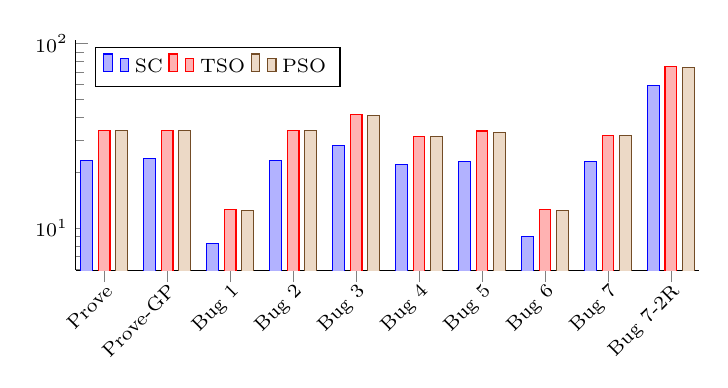
\begin{tikzpicture}
\scriptsize
\begin{axis}[
  ybar,
  bar width=0.15cm,
  height=4.5cm,
  width=9.5cm,
  axis lines*=left, % remove lines in the background
  ymode=log,
  %ylabel=Maximum memory consumption (gigabytes),
  symbolic x coords={Prove, Prove-GP, Bug 1, Bug 2, Bug 3, 
                     Bug 4, Bug 5, Bug 6, Bug 7, Bug 7-2R,
                    },
  xtick=data,
  %nodes near coords, % numbers displayed above the bars
  %every node near coord/.append style={font=\small, rotate=90, anchor=west},
  xticklabel style={
    inner sep=0pt,
    anchor=north east,
    rotate=45
  },
  %enlargelimits=0.15,
  enlarge y limits=0.15, % space relative to the height of the plot
  enlarge x limits=0.05, % space relative to the width of the plot
  legend style={
    %anchor=north, at={(0.5, -0.9)}, % legend location
    legend pos=north west,
    legend columns=-1,
    font=\scriptsize},
]

\addplot % SC
  coordinates {(Prove, 23.27) (Prove-GP, 23.90)
               (Bug 1, 8.24) (Bug 2, 23.26) (Bug 3, 28.04)
               (Bug 4, 22.18) (Bug 5, 23.02) (Bug 6, 9.03)
               (Bug 7, 22.87) (Bug 7-2R, 59.07)
              };

\addplot % TSO 
  coordinates {(Prove, 34.00) (Prove-GP, 34.00)
               (Bug 1, 12.60) (Bug 2, 34.01) (Bug 3, 41.18)
               (Bug 4, 31.49) (Bug 5, 33.65) (Bug 6, 12.59)
               (Bug 7, 31.93) (Bug 7-2R, 74.80)
              };


\addplot % PSO
  coordinates {(Prove, 33.76) (Prove-GP, 33.76)
               (Bug 1, 12.42) (Bug 2, 33.75) (Bug 3, 40.95)
               (Bug 4, 31.27) (Bug 5, 33.04) (Bug 6, 12.44)
               (Bug 7, 31.71) (Bug 7-2R, 74.51)
              };

\legend{SC, TSO, PSO}
\end{axis}
\end{tikzpicture}

\caption{Maximum Memory Consumption in Gigabytes}
\label{fig:barchart_memory}
\end{figure}

Figures~\ref{fig:barchart_sat_constr}--\ref{fig:barchart_sat_var} 
compare the formula size between SC, TSO and TSO. Comparison of 
runtime and memory can be found in Figures~\ref{fig:barchart_runtime} 
and \ref{fig:barchart_memory}. As we can see,
%Table~\ref{tab:results_cbmc} also shows that
the runtime and memory overhead for the TSO and PSO variants of a given experiment 
are quite similar.
The overheads of TSO
are slightly higher than those of PSO in all bug-injection scenarios except
for Bug 7 on which PSO had longer runtime.
However, the overhead of TSO and PSO is significantly larger than that of SC,
with up to 340\% (Bug 6 runtime) and 50\% (Bug 1 memory) increases.
The runtime was 5--19 hours and memory consumption exceeded
31\,GB in all scenarios except Bug 1 and 6.  The numbers of variables and
clauses are 37m--49m and 188m--245m, respectively, around 130\%
greater than SC.

The two-reader variant of Bug~7 has by far the longest
runtime, consuming more than 19~hours and
78~hours over SC and TSO, respectively, comparing to 9~hours and 11~hours
with one reader.  It also consumed about 75\,GB memory, more than double
the one-reader variant.  For PSO, with two reader threads CBMC's solver ran
out of memory after 85~hours whereas with one reader it completed
in less than 12~hours.  The increased overhead
is due to the
additional RCU reader's call to
\co{rcu_process_callbacks()}.
This in turn results in
more than a 125\% increase in the number of constraints, variables, and
clauses.  For example, the two-reader TSO formula has
triple the constraints and double the variables and clauses
of the one-reader case.
